\newcommand{\decktitle}{Python III - Kontrollstrukturen}

%%%%%%%%%%%%%%%%%%%%%%%%%%%%%%%%%%%%%%%%%%%%%%%%%
%
% DOCUMENT
%
%%%%%%%%%%%%%%%%%%%%%%%%%%%%%%%%%%%%%%%%%%%%%%%%%

\begin{frame}
    \subtitle{\decktitle}
    \titlepage
\end{frame}


\begin{frame}
    \frametitle{\textbf{Outline:}}
    \tableofcontents
\end{frame}

		
\section{Built-in Funktionen}
    \label{sec:builtin-func}

    \begin{frame}{Built-in Funktionen}
    
        Primär besteht die Aufgabe eines Entwicklers darin, sich konkrete oder abstrakte Lösungen zu einem bestehenden Problem zu überlegen und diese mithilfe eines Algorithmus in einer Programmiersprache umzusetzen. Häufig sind das Problem sowie die Lösung dabei so problemspezifisch, dass die Funktionalität hierfür in der gewünschten Form noch nicht existiert und deswegen vom Programmierer von Grund auf entwickelt werden muss. \\~\
        
        In der Regel sind Programme/Algorithmen aber so aufgebaut, dass komplexe Funktionalitäten aus der Komposition (Zusammensetzung) vieler einfacher Funktionen bestehen. Diese "einfachen" Funktionen sind so elementar und abstrakt, dass sie unabhängig vom konkreten Problem universell genutzt werden können. Daher ist es nicht sinnvoll, dass diese Elementarfunktionen, die sehr häufig benötigt werden, von jedem Entwickler von neuem geschrieben werden. Vielmehr enthalten die meisten Programmiersprachen bereits eine Menge verschiedener Grundfunktionen, die bereits fest in der Sprache integriert sind und daher ohne weitere Umstände von jedem Entwickler genutzt werden können. \\~\
        
        Diese Funktionen, die bereits mit der Installation des Python-Interpreters mitgeliefert werden, werden \textbf{Built-in Funktionen} genannt. 
        
    \end{frame}
    
    \begin{frame}{Built-in Funktionen}
        Python bietet eine große Zahl von Built-in Funktionen, die dem Entwickler zur Verfügung stehen, was eine schnelle und einfache Entwicklung ermöglicht. \\~\
        
        Die wichtigsten und hilfreichsten Built-in Funktionen werden im Folgenden vorgestellt. Einige dieser Built-in Funktionen sind bereits aus vorherigen Themengebieten bekannt. \\~\
        
        Eine komplette Übersicht aller eingebauten Funktionen findet sich in der offiziellen Dokumentation: \href{https://docs.python.org/3/library/functions.html}{https://docs.python.org/3/library/functions.html}
    \end{frame}    
    
    \begin{frame}[fragile]{Konvertierungsfunktionen und Konstruktoren}
        Funktionen, um Datentypenkonvertierungen (Casting) durchzuführen:
        
        \begin{itemize}
            \item \textbf{Numerische Typkonvertierungen:} \code{int(x)}, \code{float(x)}, \code{complex(x)}, \code{bool(x)}, \code{bin(x)}, ...
            
            \item \textbf{String Typkonvertierungen:} \code{str(x)}, \code{unicode(x)}, ...
            
            \item \textbf{Sequence Konstruktoren und Typkonvertierungen:} \code{list(x)}, \code{tuple(x)}, \code{range(x)}, ...
            
            \item \textbf{Map Konstruktoren und Typkonvertierungen:} \code{dict(x)}
            
            \item \textbf{Set Konstruktoren und Typkonvertierungen:} \code{set(x)}, \code{frozenset}
        \end{itemize}
    \end{frame}
    
    \begin{frame}[fragile]{Sequence Funktionen}
        Funktionen, die auf Sequence (und teilweise andere) Objekte angewendet werden können. \textbf{Das übergebene Sequence-Objekt \code{x} bleibt dabei jeweils unverändert}.
        
        \begin{itemize}
            \item \code{len(x)}: Anzahl der Elemente in der Sequence \code{x}
            
            \item \code{reversed(x)}: Erzeugt eine neue Sequence mit den gleichen Elementen in \code{x}, jedoch in umgekehrter Reihenfolge
            
            \item \code{sorted(x)}: Erzeugt eine neue Sequence mit den gleichen Elementen in \code{x}, jedoch in sortierter Reihenfolge (alphanumerische Sortierung)
            
            \item \code{sum(x)}: Erzeugt ein neues Skalar mit der Summe aller Elemente innerhalb der Sequence. Nur anwendbar auf numerische Sequence-Elemente.
            
            \item \code{zip(x)}: Erzeugt eine Sequence (zip-Objekt) von Tuples, in der jedes Tuple an Stelle $i$ das jeweils $i$-te Element der übergebenen Sequences enthält
            
\begin{pyconcode}
>>> result = zip([1,2,3], ['Alice', 'Bob', 'Carol'])
>>> print(list(result))
[(1, 'Alice'), (2, 'Bob'), (3, 'Carol')]
\end{pyconcode}            
        \end{itemize}
    \end{frame}
    
    \begin{frame}[fragile]{Input \& Output (I)}
        Elementare Funktionen zur Interaktion zwischen Mensch und System bzw. zur Eingabe und Ausgabe von Daten:
        
        \begin{itemize}
            \item \textbf{Ausgabe:} Um Werte (Numerische Werte, Strings, ...) auf der Standardausgabe auszugeben, wird \code{print()} verwendet.
            
            \item \textbf{Eingabe:} Analog existiert eine Funktion zur Eingabe von Werten: \code{input()}. Mithilfe dieser Funktionen können Werte von der Standardeingabe eingelesen werden, um beispielsweise Nutzereingaben abzufragen. Der \code{input()}-Funktion kann auch ein Parameter übergeben werden. Dabei handelt es sich um einen String, der dem Nutzer vor der Eingabe angezeigt wird ("Prompt"). Die Eingabe kann anschließend in einer Variable gespeichert werden.
            
\begin{pyconcode}
>>> x = input()
<<< Hello world
>>> print(x)
Hello world

>>> x = input("Please enter text: ")
<<< Bitte Text eingeben: Hello world
>>> print(x)
Hello world
\end{pyconcode}            
        \end{itemize}
    \end{frame}
    
    \begin{frame}[fragile]{Input \& Output (II)}
        \begin{alertblock}{Achtung}
            Da der Python-Interpreter nicht weiß, welchen Datentyp die Eingabe besitzen soll, wird die Eingabe standardmäßig als Strings eingelesen und gespeichert. 
            
            Soll jedoch ein anderer Datentyp eingelesen werden, z.B. eine Ganzzahl, muss der Wert nach der Eingabe mit der entsprechenden Funktion konvertiert werden
            
\begin{pyconcode}
>>> age = input("Please enter your age: ")
<<< Please enter your age: 20
>>> type(age)
<class 'str'>
>>> age = int(age)
>>> type(age)
<class 'int'>
\end{pyconcode}
        \end{alertblock}
    \end{frame}
    
    \begin{frame}[fragile]{Input \& Output (III)}
        \begin{itemize}
            \item \textbf{Eingabe:} Neben der Eingabe von Text können auch Dateien eingelesen werden. Hierzu steht die \code{open()}-Funktion zur Verfügung. Diese Funktion erwartet den Dateinamen (ggfs. inkl. Dateipfad, falls sich die Datei nicht im aktuellen Verzeichnis befindet.). Außerdem muss ggfs. der Modus angegeben werden: \code{'r'}, falls die Datei nur zum Lesen (Read) geöffnet wird, \code{'w'} zum Schreiben (Write)
            
\begin{pyconcode}
>>> content = open("main.py", "r")
>>> type(content)
<class '_io.TextIOWrapper'>
>>> lines = content.readlines()
>>> type(lines)
<class 'list'>
>>> print(lines)
['print("Hello world")\n']
\end{pyconcode}
        \end{itemize}
    \end{frame}
    
    \begin{subsection}{Aufgaben}
            \begin{frame}[fragile, allowframebreaks]{Aufgaben}
                \begin{enumerate}
                    \item Wozu gibt es die Built-in Funktionen?
                    \item Was ist nötig, um die Built-in Funktionen zu nutzen?
                    \item Es existieren zwei Tuples, die jeweils unterschiedliche Namen enthalten. Wie können daraus ganz einfach jeweils Paare von zwei Namen erzeugt werden?
                    \item Wo erscheint die Ausgabe von \code{print()}?
                    \item Was muss bei der \code{input()}-Funktion beachtet werden? Worin liegt der Unterschied zur \code{open()}-Funktion?
                    
                    \item Wie können mithilfe der \code{open()}-Funktion Dateiinhalte gelesen werden, die sich außerhalb des aktuellen Verzeichnisses befinden?
                    
                    \begin{block}{Hinweis}
                        Hinweis: Weitere Übungsaufgaben zum Themenblock 'Built-in Funktionen' finden sie im entsprechenden Übungsblatt.
                    \end{block}
                    
                    
                    
                \end{enumerate}
            \end{frame}
        \end{subsection}
    
\section{Steueranweisungen}
    
    \begin{frame}{Steueranweisungen}
        Mit den bis hierhin gelernten Funktionalitäten ist es bereits möglich, grundlegende und erweiterte Abläufe in Python umzusetzen. Von den eingangs vorgestellten Grundeigenschaften einer Programmiersprache sind nun bereits folgende Charakteristiken bekannt: \\~\
        
        \begin{itemize}
            \item Ein- und Ausgabe (\code{print()} und \code{input()} bzw. \code{open()})
            \item Variablendeklaration
            \item Mathematische Grundoperationen
            \item Zeichenkettenverarbeitung
        \end{itemize}
        
        Als letzte noch fehlende Eigenschaft werden im folgenden die unterschiedlichen Steueranweisungen vorgestellt und erläutert.
    \end{frame}
    
    \begin{frame}{Steueranweisungen}
        Mithilfe von Steueranweisungen kann der Ablauf eines Programms gesteuert werden. Somit ist es nun möglich, dass der Code nicht nur ausschließlich "von oben nach unten" durchläuft, sondern unterschiedliche Wege nehmen kann, an eine andere Stelle springt und dort fortgesetzt wird oder aber bestimmte Anweisungen mehrmals ausgeführt werden. \\~\
        
        Dies ermöglicht eine effiziente Programmierung, mit der der statische Ablauf ohne spezifische Anpassungen in eine dynamische, flexiblere Arbeitsweise wechselt. \\~\
        
        Es gibt unterschiedliche Arten von Steueranweisungen, die unterschiedliche Zwecke erfüllen. Die wichtigsten Steueranweisungen werden im Folgenden erläutert. Diese sind in fast jeder modernen Programmiersprache vorhanden, jedoch gibt es teilweise mehr oder weniger starke Abweichungen in der Syntax.
    \end{frame}
    
    \begin{subsection}{Conditionals}
        
        \begin{frame}{Conditionals}
            Die einfachste Art einer Steueranweisung sind \textbf{Conditionals} bzw. \textbf{Bedingte Anweisungen} oder auch \textbf{Verzweigungen} genannt. \\~\
            
            Hiermit kann der Ablauf des Codes beeinflusst werden, indem anhand von klar definierten Bedingungen unterschiedliche Codeabschnitte ausgeführt werden können. \\~\
            
            Conditionals sind eng mit den booleschen Werten verknüpft, da die Bedingungen jeweils als Wahrheitswert ausgewertet werden und daher entweder \code{True} oder \code{False} ergeben. \\~\
            
            Bedingte Anweisungen sind insbesondere dann unabdingbar, wenn mit dynamischen Informationen, wie etwa Dateneinspeisungen von anderen System oder Nutzereingaben gearbeitet wird, da hier die exakten Daten zur Zeit der Programmierung noch nicht bekannt sind und daher der Programmablauf dynamisch angepasst werden muss.
            
        \end{frame}
        
        \begin{frame}{if (I)}
            Die Conditionals folgen immer einem "Wenn Dann"-Schema, d.h. \textbf{wenn} die Bedingung wahr ist, \textbf{dann} wird der entsprechende Codeabschnitt ausgeführt. Andernfalls wird der Codeabschnitt übersprungen. \\~\
            
            Dementsprechend existiert in Python das Schlüsselwort \code{if}, mit dem eine Bedingung eingeleitet und entsprechend ausgewertet wird.\\~\
            
            Der Programmablauf folgt dabei der exemplarischen Darstellung \ref{fig:if}, die auf der nächsten Seite abgebildet ist.
        \end{frame}
        
        \begin{frame}{if (II)}
            \begin{figure}
                \centering
                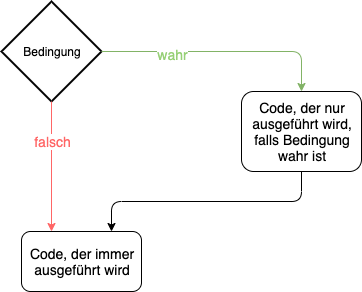
\includegraphics[width=0.7\linewidth, keepaspectratio]{chapters/09_python3_control_flow/figures/if.png}
                \caption{Der Programmablauf mit einer Verzweigung}
                \label{fig:if}
            \end{figure}
        \end{frame}
    
        \begin{frame}[fragile]{if (III)}
            Die Syntax sieht dabei folgendermaßen aus:
            
\begin{pythoncode}
if <Bedingung>:
    # Anweisungen, die ausgeführt werden, wenn Bedingung wahr ist

# Anweisungen, die immer ausgeführt werden
\end{pythoncode}

            Hierbei sind mehrere Dinge zu beachten:
            
            \begin{itemize}
                \item Die Bedingung muss immer entweder \code{True} oder \code{False} sein. Auch Verknüpfungen von logischen Aussagen mit z.B. \code{and} sind zulässig
                \item Nach der Bedingung folgt immer ein Doppelpunkt. Hiermit wird verdeutlicht, dass im Folgenden die Anweisungen stehen, die ausgeführt werden, falls die Bedingung wahr ist
                \item Diese Bedingungen \textbf{müssen um eine Ebene} eingerückt sein, um den Anfang und das Ende des Blocks zu kennzeichnen
                \item Anweisungen außerhalb der if-Clause werden wieder ausgerückt
            \end{itemize}
        
        \end{frame}
        
        \begin{frame}[fragile]{if (IV)}
            
            \begin{exampleblock}{Beispiel}
            
\begin{pythoncode}
age = int(input("Bitte Alter eingeben: "))
if age >= 18:
    print("Der Nutzer ist volljährig")

print("Der Nutzer ist " + str(age) + " Jahre alt")
\end{pythoncode}

            \end{exampleblock}
        \end{frame}
        
        \begin{frame}[fragile]{if (V)}
            
            \begin{alertblock}{Achtung}
            
                Der interaktive Interpreter wertet im Normalfall jede Eingabe des Nutzer direkt aus. Nachdem der Nutzer aber eine if-Clause eingegeben hat, kann diese der Interpreter noch nicht ausführen, da er noch die Anweisungen erwartet, die ausgeführt werden sollen, falls die Bedingung wahr ist. Aus diesem Grund zeigt der Interpreter nach Eingabe der if-Clause zunächst \code{...} an, wodurch der Nutzer nun seine Anweisungen eingeben kann. Soll die if-Clause abgeschlossen werden, muss der Nutzer dies erneut mit der Enter-Taste bestätigen.

            \end{alertblock}
        \end{frame}
        
        \begin{frame}[fragile]{if-else (I)}
            In vielen Fällen soll nicht nur überprüft werden, ob eine Bedingung wahr ist, sondern auch Anweisungen ausgeführt werden, wenn dies nicht der Fall ist. Eine Möglichkeit besteht darin, die verneinte Aussage erneut zu überprüfen:
            
\begin{pythoncode}
age = int(input("Bitte Alter eingeben: "))
if age >= 18:
    print("Der Nutzer ist volljährig")

if age < 18:
    print("Der Nutzer ist nicht volljährig")
\end{pythoncode}

            Da dieses Vorgehen jedoch redundant ist gibt es hierfür eine häufig verwendete Kurzform: Das \textbf{if-else} Konstrukt 
                
        \end{frame}
        
        \begin{frame}[fragile]{if-else (II)}
            Mithilfe von \textbf{if-else} kann zunächst überprüft werden, ob eine Aussage wahr ist und dementsprechend Anweisungen ausgeführt werden. Ist die Aussage jedoch nicht wahr, werden die Anweisungen ausgeführt, die in der \code{else}-Clause enthalten sind \\~\
            
            Der Programmablauf folgt dabei der exemplarischen Darstellung \ref{fig:if-else}, die auf der nächsten Seite abgebildet ist.
        
        \end{frame}
        
         \begin{frame}[fragile]{if-else (III)}
            \begin{figure}
                \centering
                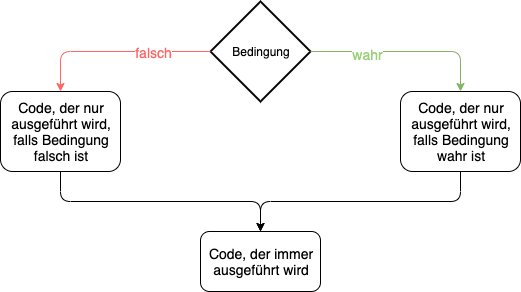
\includegraphics[width=0.7\linewidth, keepaspectratio]{chapters/09_python3_control_flow/figures/if-else.png}
                \caption{Der Programmablauf mit einer if-else Verzweigung}
                \label{fig:if-else}
            \end{figure}
         \end{frame}
         
        \begin{frame}[fragile]{if-else (IV)}
            Die Syntax sieht dabei folgendermaßen aus:
            
\begin{pythoncode}
if <Bedingung>:
    # Anweisungen, die ausgeführt werden, wenn Bedingung wahr ist
else:
    # Anweisungen, die ausgeführt werden, wenn Bedingung falsch ist
    
# Anweisungen, die immer ausgeführt werden
\end{pythoncode}

            Hierbei sind mehrere Dinge zu beachten:
            
            \begin{itemize}
                \item Bei der else-Clause wird nie eine Bedingung überprüft, da diese automatisch ausgeführt wird, falls die Bedingung der if-Clause zu \code{False} auswertet.
                \item Es wird \textbf{entweder} die if-Clause oder \textbf{oder} die else-Clause ausgeführt. Es ist nicht möglich, dass keine der beiden oder  beide gleichzeitig ausgeführt werden.
                \item Nach den Anweisungen der if-Clause muss eine Ausrückung erfolgen, da hier ein neuer Block beginnt. Die Anweisungen der else-Clause werden dann wieder eingerückt.
                \item Eine else-Clause ist immer optional
            \end{itemize}
        
        \end{frame}
        
        \begin{frame}[fragile]{if-else (V)}
            
            \begin{exampleblock}{Beispiel}
            
\begin{pythoncode}
age = int(input("Bitte Alter eingeben: "))
if age >= 18:
    print("Der Nutzer ist volljährig")
else: 
    print("Der Nutzer ist nicht volljährig")

print("Der Nutzer ist " + str(age) + " Jahre alt")
\end{pythoncode}

            \end{exampleblock}
        \end{frame}
        
        
        \begin{frame}[fragile]{if-elif-else (I)}
            Um komplexere Abfragen noch einfacher umsetzen zu können, gibt es eine Erweiterung des \code{if} bzw. \code{if-else} Konstrukts:\\~\
            
            Mithilfe von else-if (Keyword: \code{elif}) können beliebig viele Aussagen auf ihren Wahrheitswert überprüft werden. Sobald eine dieser Aussagen wahr ist, werden die entsprechenden Anweisungen ausgeführt. Die nachfolgenden \code{elif}-Clauses werden dann nicht mehr überprüft, auch die \code{else}-Anweisungen werden dann nicht mehr ausgeführt. \\~\
            
            Der Programmablauf folgt dabei der exemplarischen Darstellung \ref{fig:elif}, die auf der nächsten Seite abgebildet ist.
        \end{frame}
        
        \begin{frame}[fragile]{if-elif-else (II)}
            \begin{figure}
                \centering
                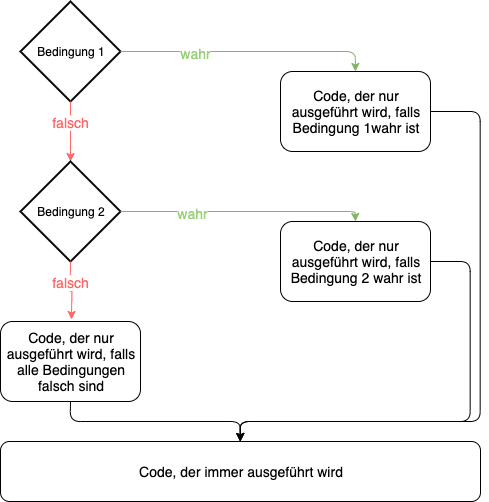
\includegraphics[width=0.7\linewidth,height=0.7\textheight,keepaspectratio]{chapters/09_python3_control_flow/figures/elif.png}
                \caption{Der Programmablauf mit einer if-elif-else Verzweigung}
                \label{fig:elif}
            \end{figure}
         \end{frame}
         
         \begin{frame}[fragile]{if-elif-else (III)}
            Die Syntax sieht dabei folgendermaßen aus:
            
\begin{pythoncode}
if <Bedingung 1>:
    # Anweisungen, die ausgeführt werden, wenn Bedingung 1 wahr ist
elif <Bedingung 2>:
    # Anweisungen, die ausgeführt werden, wenn Bedingung 2 wahr und Bedingung 1 falsch ist
elif <Bedingung 3>:
    # Anweisungen, die ausgeführt werden, wenn Bedingung 3 wahr und Bedingung 1 und Bedingung 2 falsch sind
else:
    # Anweisungen, die ausgeführt werden, wenn alle Bedingungen falsch sind
    
# Anweisungen, die immer ausgeführt werden
\end{pythoncode}

            Hierbei sind mehrere Dinge zu beachten:
            
            \begin{itemize}
                \item Es werden die Bedingungen der Reihe nach geprüft. Die Anweisungen der ersten Bedingung, die \code{True} ergibt, werden ausgeführt, die restlichen \code{elif} bzw. \code{else}-Statements ignoriert.
                \item Wertet keine der \code{if} oder \code{elif}-Clauses zu \code{True} aus, wird die \code{else}-Clause ausgeführt (falls vorhanden)
                \item Auch hier ist die \code{else}-Clause optional
            \end{itemize}
        
        \end{frame}
        
        \begin{frame}[fragile]{if-elif-else (IV)}
            
            \begin{exampleblock}{Beispiel}
            
\begin{pythoncode}
age = int(input("Bitte Alter eingeben: "))
if age > 18:
    print("Der Nutzer ist volljährig")
elif age == 18:
    print("Der Nutzer ist dieses Jahr volljährig geworden.")
else: 
    print("Der Nutzer ist nicht volljährig")

print("Der Nutzer ist " + str(age) + " Jahre alt")
\end{pythoncode}

            \end{exampleblock}
        \end{frame}
        
        \begin{frame}{Verschachtelte Conditionals (I)}
            Bedingte Anweisungsblöcke können auch verschachtelt werden, d.h. in einer \code{if}, \code{elif} oder \code{else}-Clause können wiederum weitere bedingte Anweisungen enthalten sein.  \\~\
            
            Eine (praktische) Maximalzahl an erlaubten Verschachtelungen gibt es nicht.
            
        \end{frame}
        
        \begin{frame}{Verschachtelte Conditionals (II)}
            \begin{alertblock}{Achtung}
                Für jeden Anweisungsblock muss der Code um eine Ebene eingerückt werden. Enthält also beispielsweise eine \code{if}-Clause eine weitere \code{if}-Clause, muss der Code um 2 Ebenen eingerückt werden.
            \end{alertblock}
        \end{frame}
        
          \begin{frame}[fragile]{Verschachtelte Conditionals (III)}
            \begin{exampleblock}{Beispiel}
\begin{pythoncode}
username = int(input("Bitte Benutzername eingeben: "))
password = input("Bitte Passwort eingeben: ")

if username in  ["Alice", "Bob", "Carol"]:
    if len(password) < 6:
        print("Das Passwort ist unsicher")
    else:
        print("Der Nutzer " + username + " existiert und das Passwort ist sicher")
else:
    print("Der Nutzername ist nicht bekannt")
\end{pythoncode}
            \end{exampleblock}
        \end{frame}
        
    
    \begin{subsubsection}{Aufgaben}
        \begin{frame}[fragile, allowframebreaks]{Aufgaben}
            \begin{enumerate}
                \item Wofür werden Conditionals benötigt?
                \item Kann jede Funktionalität der Conditionals auch ohne Conditionals genutzt werden?
                \item Warum gibt es Einrückungen?
                \item Können bei Conditionals auch andere Datenwerte als boolesche Werte auf Wahrheit getestet werden?
                \item Warum werden bei else-Clauses keine Bedingungen abgefragt?
                \item Wie viele Anweisungen darf eine if-Clause besitzen?
                \item Kann eine \code{elif}-Clause auch anders ausgedrückt werden?
                \item Werden stets alle Bedingungen eines if-elif-else-Konstrukts überprüft?
                \item Was muss bei der Verschachtelung von Conditionals beachtet werden?
                
               \begin{block}{Hinweis}
                Hinweis: Weitere Übungsaufgaben zum Themenblock 'Conditionals' finden sie im entsprechenden Übungsblatt.
            \end{block}
            
            \end{enumerate}
        \end{frame}
    \end{subsubsection}
% Kurzschreibweise
    \end{subsection}
    
    \begin{subsection}{Schleifen}
        
        \begin{frame}{Schleifen (I)}
            Schleifen stellen in der Programmierung ein wichtiges Werkzeug dar, das zu einer effizienten, schnellen und einfachen Entwicklung beiträgt. \\~\
            
            Der Sinn einer Schleife besteht darin, eine Anweisung mehrmals auszuführen, ohne jede einzelne dieser Anweisungen "hartgecoded" (also explizit aufgeführt) in den Programmcode zu schreiben. \\~\
            
            Schleifen werden häufig auch \textit{Loops} genannt.
        \end{frame}
        
        \begin{frame}[fragile]{Schleifen (II)}
        
            Im Folgenden ist ein Beispiel dargestellt, wie alle Elemente einer Liste (ohne Schleife) der Reihe nach ausgegeben werden: 
            
            \begin{exampleblock}{Beispiel}
\begin{pythoncode}
names = ['Alice', 'Bob', 'Carol', 'Dave']
index = 0

print(names[index])
index = index+1
print(names[index])
index = index+1
print(names[index])
index = index+1
print(names[index])
\end{pythoncode}            
            \end{exampleblock}
            
            Hier ist deutlich zu erkennen, dass diese Art der Ausgabe aller Listenelemente sehr ineffizient ist. Insbesondere bei längeren Listen ist eine solche Vorgehensweise unpraktikabel.
        \end{frame}
        
        \begin{frame}[fragile]{Schleifen (III)}
            Abhilfe hierfür schaffen Schleifen, da mit diesen wiederkehrende Anweisungen nur einmal angegeben werden müssen und diese dann beliebig oft ausgeführt werden kann. \\~\
            
            Generell gibt es in Python zwei Arten von Schleifen: \code{while}-Schleifen und \code{for}-Schleifen. \\~\
            
            Die Funktionsweise der beiden Schleifentypen ist sehr ähnlich, mit beiden Arten können jeweils die gleichen Funktionalitäten umgesetzt werden. Jedoch gibt es feine Unterschiede, durch die sich \code{for} und \code{while}-Schleifen unterscheiden und sich je nach Anwendungsfall der eine oder der andere Typ eher anbietet.
        \end{frame}
        
        \begin{frame}[fragile]{Schleifen (IV)}
            Alle Schleifen folgen dem gleichen Ablauf:
                
                \begin{enumerate}
                    \item Prüfe, ob die Abbruchbedingung der Schleife erfüllt ist. Falls nicht, gehe zu Schritt 2
                    \item Führe die Anweisungen aus, die im Schleifenrumpf enthalten sind. Anschließend gehe zu Schritt 1.
                \end{enumerate}
        \end{frame}
        
        
        
        \begin{frame}[fragile]{while (I)}
            Mithilfe von \code{while}-Schleifen können Anweisungen solange ausgeführt werden, solange die Anweisung im Schleifenkopf wahr ist. \\~\
            
            Das bedeutet, dass der Entwickler sich zunächst überlegen muss, was das \textbf{Abbruchkriterium} ist.
            
            Die Syntax des \code{while}-Loops sieht folgendermaßen aus:
            
\begin{pythoncode}
while <Bedingung>:
    # Anweisungen, die ausgeführt werden, solange die Bedingung wahr ist

# Anweisungen, die ausgeführt werden, nachdem die Schleife beendet wurde / durchgelaufen ist
\end{pythoncode}
        \end{frame}
        
        \begin{frame}{while (II)}
            Die Bedingung, die im Schleifenkopf angegeben wird, muss stets ein boolescher Ausdruck sein, die entweder \code{True} oder \code{False} ergibt. Sobald die Anweisung zu \code{False} ausgewertet wird, ist die Schleife beendet und der Codeablauf wird fortgesetzt. \\~\
            
            \code{while}-Schleifen werden i.d.R. dann verwendet, wenn eine Anweisung bestimmt oft (x Mal) ausgeführt werden soll.
            
        \end{frame}
        
        \begin{frame}{while (III)}
            \begin{alertblock}{Achtung}
                \code{while}-Schleifen sind \textbf{kopfgesteuerte} Schleifen. Das bedeutet, dass die Abbruchbedingung \textbf{vor} jedem Schleifendurchgang überprüft wird. Wenn die Bedingung \code{False} ist, wird der nächste Schleifendurchgang nicht mehr ausgeführt.
                Es gibt auch \textbf{fußgesteuerte} Schleifen, bei denen \textbf{nach} jedem Durchgang die Bedingung geprüft wird und abhängig davon der nächste Schleifendurchgang gestartet wird. \\~\
                
                Das hat zur Folge, dass fußgesteuerte Schleifen mindestens einmal durchlaufen werden, bei kopfgesteuerten Schleifen ist es auch möglich, dass kein Schleifendurchlauf stattfindet.
            \end{alertblock}
        \end{frame}
        
        \begin{frame}[fragile]{while (IV)}
                \begin{exampleblock}{Beispiel}
                
                Im folgenden Codeausschnitt sollen die Zahlen von 0 bis 5 in absteigender Reihenfolge ausgegeben werden, ohne die expliziten Werte anzugeben:
\begin{pyconcode}
>>> i = 5
>>> while i >= 0:
>>>     print(i)
>>>     i = i-1

5
4
3
2
1
0
\end{pyconcode}                
                \end{exampleblock}
        \end{frame}
        
        \begin{frame}[fragile]{while (V)}
            \begin{alertblock}{Achtung}
                Die Anweisung \code{i = i-1} im vorherigen Beispiel ist sehr wichtig, da hierdurch die Variable \code{i} um den Wert 1 verringert wird. Wird diese Anweisung vergessen, wird bei jedem Schleifendurchgang überprüft, ob \code{i>0} wahr ist. Da sich \code{i} nicht ändert, wird stets überprüft ob \code{5 > 0} wahr ist, was immer der Fall ist. Dies hat eine \textbf{Endlosschleife} zur Folge, da die Abbruchbedingung nie erreicht wird.
            \end{alertblock}
        \end{frame}
        
        \begin{frame}{for (I)}
        
            Neben den \code{while} Schleifen gibt es noch eine weitere Schleifenart: Die \code{for} Schleife. \\~\
            
            Anders als \code{while} Schleifen sind \code{for} Schleifen nicht zähler- sondern elementbasiert. Der Vorteil liegt darin, dass so ein Durchlaufen (Iterieren) aller Elemente einer Liste oder listenähnlichen Struktur sehr einfach ist. \\~\
            
            Die Gefahr, dass der Entwickler vergisst, eine Zählvariable zu in-/dekrementieren und so eine Endlosschleife zu erzeugen, sinkt.
            
        \end{frame}
        
        
        \begin{frame}[fragile]{for (II)}
            Die Syntax einer \code{for}-Schleife ist folgendermaßen:
            
\begin{pythoncode}
for <Elementvariable> in <Sequence>:
    # Anweisungen, die für jedes Element der Sequence ausgeführt werden

# Anweisungen, die nach Durchlaufen der Schleife ausgeführt werden
\end{pythoncode} \\~\

            Bei \code{for} Schleifen wird über jedes Element der Sequenz iteriert, welches automatisch einer Variablen (oben \code{<Elementvariable>}) zugewiesen wird.\\~\
            
            Im Gegensatz zur \code{while} Schleife muss der Entwickler hier also keine explizite Abbruchbedingung angeben, sondern der Schleifendurchlauf endet, wenn alle Elemente der Sequenz ein Mal durchlaufen wurden.
        \end{frame}
        
        \begin{frame}[fragile]{for (III)}
            \begin{exampleblock}{Beispiel}
            
            Im folgenden Codeausschnitt sollen die Namen, die in der Liste enthalten sind, ausgegeben werden:
            
\begin{pythoncode}
names = ['Alice', 'Bob', 'Carol', 'Eve', 'Dave']

for name in names:
    print(name)

Alice
Bob
Carol
Eve
Dave
\end{pythoncode}

            Der Name der Variablen \code{name} als Variable für das jeweilige Listenelement kann frei gewählt werden \footnote{solange er den Regeln der Variablenbenennung entspricht}
            
            \end{exampleblock}
        \end{frame}
        
        \begin{frame}[fragile]{range (I)}
            Eine der am häufigsten im Zusammenhang mit der \code{for} Schleife genutzten Built-In Funktionen ist \code{range()}. \\~\
            
            Mithilfe von \code{range()} können einfach Sequenzen von Zahlen erzeugt werden. \\~\
            
            Wird der \code{range()}-Funktion nur ein Parameter übergeben, wird eine Sequenz von Zahlen von 0 bis zur entsprechenden Zahl erzeugt:
            
\begin{pyconcode}
>>> intervall = range(5)
>>> type(intervall)
<class 'range'>

>>> intervall_list = list(intervall)
>>> type(intervall_list)
<class 'list'>
>>> print(intervall_list)
[0, 1, 2, 3, 4]
\end{pyconcode}

        \end{frame}
        
        \begin{frame}[fragile]{range (II)}
             Werden der \code{range()}-Funktion 2 Parameter übergeben, wird eine Sequenz von Zahlen vom Anfangswert (Parameter 1) bis zum Endwert (Parameter 2) erzeugt:

\begin{pythoncode}
intervall = range(5,12)
for number in intervall:
    print(number)

5
6
7
8
9
10
11
\end{pythoncode}             
        \end{frame}
        
        \begin{frame}[fragile]{range (III)}
             Werden der \code{range()}-Funktion 3 Parameter übergeben, wird eine Sequenz von Zahlen vom Anfangswert (Parameter 1) bis zum Endwert (Parameter 2) mit einer Schrittweite (Parameter 3) erzeugt:

\begin{pythoncode}
intervall = range(5,12,2)
for number in intervall:
    print(number)

5
7
9
11
\end{pythoncode}        

            Wird keine Schrittweite angegeben, wird automatisch der Standartwert 1 verwendet.
             
        \end{frame}
        
        \begin{frame}{range (IV)}
        
           \begin{alertblock}{Achtung}
                Bei der \code{range()}-Funktion ist der Anfangswert stets inklusiv, der Endwert immer exklusiv. \code{range(2,7)} beinhaltet also alle Zahlen zwischen 2 und 6.
            \end{alertblock}  
        \end{frame}
        
        \begin{frame}[fragile]{range (V)}
        
            Die \code{range()}-Funktion wird häufig in Kombination mit der \code{for} Schleife genutzt, da so die Funktionalität einer zählerbasierten \code{while} Schleife nachgebildet werden kann, ohne sich um die Initialisierung und Inkrementierung des Zählers kümmern zu müssen.
            
            \begin{exampleblock}{Beispiel}
                Mit der folgenden \code{while} Schleife werden die Zahlen von 1 - 20 ausgegeben:
                
\begin{pythoncode}
i = 1
while i<=20:
    print(i)
    i = i+1
\end{pythoncode}
                Die selbe Funktionalität kann mit folgender \code{for} Schleife in Kombination einfacher und übersichtlicher umgesetzt werden:

\begin{pythoncode}
for i in range(1, 21):
    print(i)
\end{pythoncode}               
                
            \end{exampleblock}
        \end{frame}

            
        
        
        \begin{frame}{continue - Iterationsabbruch (I)}
            Es gibt zwei Hilfsanweisungen, die bei der Entwicklung von Schleifen hilfreich sein können. Hierzu gehört \code{continue}.\\~\
            
            Die \code{continue} Anweisung wird genutzt, falls der aktuelle Iterationsdurchgang abgebrochen werden und mit dem nächsten Iterationsdurchgang weitergemacht werden soll (solange die Abbruchbedingung nicht erfüllt ist). \\~\
            
            Oft wird die \code{continue}-Anweisung zu den schlechten Codepraktiken gezählt, da es deutlich schwieriger werden kann, als Mensch den Programmablauf nachzuvollziehen. Aus diesem Grund sollte auf \code{continue} verzichtet werden falls möglich
        \end{frame}
        
        \begin{frame}[fragile]{continue - Iterationsabbruch (II)}
            
            \begin{exampleblock}{Beispiel}
                Im folgenden Beispiel wird für die Zahlen von 2 - 10 überprüft, ob sie gerade oder ungerade sind:
                
\begin{pythoncode}
for num in range(2, 10):
    if num % 2 == 0:
        print("Gerade Zahl gefunden")
        continue
    print("Ungerade Zahl gefunden")
\end{pythoncode}
                
                \textbf{Dieser Codeausschnitt soll lediglich die Funktionsweise von \code{continue} verdeutlichen. Der abgebildete Code sollte so nicht verwendet werden, da er unnötig umständlich ist. Eine einfachere und bessere Variante stellt hier eine Implementierung mit if-else dar.}
            \end{exampleblock}
        \end{frame}
        
        \begin{frame}{break - Schleifenabbruch (I)}
            Neben \code{continue} gibt es noch eine weitere Hilfsanweisung:  \code{break}.\\~\
            
            Die \code{break} Anweisung wird genutzt, um das Durchlaufen der Schleife abzubrechen, auch wenn die Abbruchbedingung noch nicht erfüllt ist. Im Gegensatz zu \code{continue} wird also nicht nur die aktuelle Iteration, sondern die komplette Schleife abgebrochen.  \\~\
            
            Auch \code{break} sollte nur genutzt werden, wenn die Anweisung wirklich benötigt wird, andernfalls sollten eindeutigere Codeumsetzungen bevorzugt werden.
        \end{frame}
        
        \begin{frame}[fragile]{break - Schleifenabbruch (II)}
            
            \begin{exampleblock}{Beispiel}
                Im folgenden Beispiel wird für die Zahlen ab 100 überprüft, ob sie durch 7 teilbar sind. Falls das der Fall ist, wird die Schleife abgebrochen:
                
\begin{pythoncode}
index = 100
divider = 7
while True:
    if index % divider == 0:
        print(str(index) + " ist teilbar durch " + str(divider))
        break
    else:
        print(str(index) + " ist nicht teilbar durch " + str(divider))
        index = index +1
\end{pythoncode}
            
            \end{exampleblock}
        \end{frame}

        \begin{subsubsection}{Aufgaben}
            \begin{frame}[fragile, allowframebreaks]{Aufgaben}
                \begin{enumerate}
                    \item Wofür sind Schleifen hilfreich?
                    \item Welche Arten von Schleifen gibt es? Was sind die Unterschiede?
                    \item Welche kopfgesteuerten bzw. fußgesteuerten Schleifen gibt es in Python?
                    \item Wann werden primär \code{while} und wann \code{for} Schleifen genutzt?
                    \item Was muss bei \code{while} Schleifen unbedingt beachtet werden? Warum ist das bei \code{for} Schleifen nicht relevant?
                    
                    \item Welche Funktionalität bietet die \code{range()}-Funktion?
                    \item Warum wird beim Erzeugen einer Range eine Variable des Typs \code{range} und nicht \code{list} erzeugt?
                    \item Was muss beim Erzeugen einer \code{range} beim Start- und Endwert beachtet werden?
                    \item Was ist das Ergebnis der Anweisung \code{list(range(20,0,-2))}?
                    
                    \item Wozu wird \code{continue} genutzt und warum sollte es vermieden werden?
                
                    
                \end{enumerate}
            \end{frame}
        \end{subsubsection}
    \end{subsection}
    
    
\section{Funktionen}
    
    \begin{frame}{Funktionen}
        Funktionen gehören zu den Grundkonzepten einer Programmiersprache und sind in so gut wie allen Programmiersprachen vorhanden und verwendbar. \~\\
        
        Sie stellen ein wichtiges Werkzeug dar, um den Code zu strukturieren, Funktionalitäten zusammenzufassen und Codewiederholungen zu vermeiden. 
        
        Da die Lesbarkeit und die übersichtliche Strukturierung von Code in Python eine wichtige Rolle einnimmt (siehe \textit{The Zen of Python} bzw. \textit{Computer Programming for Everybody} (Foliensatz \textit{Python 1})), nehmen die Funktionen hier eine wichtige Rolle ein. \\~\
        
        Darüber hinaus trägt eine klare Strukturierung und Aufteilung des Codes zu einer guten Codequalität bei, die es ermöglicht, Fehler schneller zu finden und den Codeablauf leichter zu beschreiben.
    \end{frame}
    
    \begin{frame}{Bereits bekannte Funktionen}
        In Abs. \ref{sec:builtin-func} wurden bereits einige Funktionen vorgestellt, die in Python standardmäßig enthalten sind und ohne weiteres aufrufbar sind. Python bietet im Gegensatz zu einigen anderen Programmiersprachen einen großen Umfang an Built-in Funktionen, die in vielen Fällen sehr praktisch sein können. \\~\
        
        Beispielsweise gehören hierzu die Ein- / Ausgabefunktionen \code{input()} und \code{print()}. Da diese Funktionalitäten sehr häufig benötigt werden, wäre es sinnlos, wenn jeder Entwickler sie jedes Mal aufs Neue implementieren müsste.
    \end{frame}
    
    \begin{frame}{Eigene Funktionen}
        Da Built-in Funktionen nur die häufigsten und gebräuchlichsten Anwendungsfälle abdecken, existieren für spezifische Problemstellungen keine standardmäßigen Funktionen im Python-Interpreter. Diese müssen dann vom Programmierer selbst entwickelt werden. \\~\
        
        Häufig werden aber auch innerhalb eines Problems ähnliche Funktionalitäten mehrmals benötigt, sodass Funktionen, die vom Entwickler einmal geschrieben wurde, an unterschiedlichen Stellen im Programmcode wiederverwendet werden können.
    \end{frame}
    
    \begin{frame}{Deklaration vs. Aufruf}
    
        Bei der Entwicklung bzw. Verwendung von Funktionen müssen zwei Fälle getrennt bzw. unterschieden werden, die bei der Implementierung von Funktionen von Bedeutung sind:\\~\
    
        
        \begin{columns}[T] % align columns
            \begin{column}{.48\textwidth}
                \textbf{Deklaration/Definition von Funktionen} 
                
                    Bevor Funktionen verwendet werden können, müssen sie zunächst definiert bzw. deklariert werden. Hierbei wird beschrieben, wie die Funktion heißt, welche Parameter sie erwartet, welche Anweisung sie ausführen soll und welche Werte sie zurückgibt.
                    
                    Allein durch die Deklaration wird sie jedoch noch nicht ausgeführt, hier wird sie lediglich \textbf{beschrieben}.
            \end{column}%
            \hfill%
            \begin{column}{.48\textwidth}
                \textbf{Aufruf von Funktionen}
                
                Erst nachdem Funktionen definiert wurden, können sie auch \textbf{ausgeführt} werden. Ein Funktionsaufruf kann sich an komplett anderer Stelle befinden als die entspr. Definition. Wichtig ist aber, dass sich die Funktion im gleichen Scope befindet. Durch den Funktionsaufruf werden der Funktion die benötigten Parameter übergeben, anschließend werden die Anweisungen ausgeführt und letztendlich ein oder mehrere Werte zurückgegeben.
            \end{column}%
        \end{columns}
    \end{frame}
    
    \begin{frame}{Funktionsdefinition (I)}
    
        Eine Funktionsdefinition besteht aus zwei Teilen:\\~\
        
        Eine Funktion beginnt immer mit dem \textbf{Funktionskopf}. Um zu kennzeichnen, dass eine Funktionsdefinition folgt, beginnt dieser immer mit dem \code{def} Schlüsselwort. 
        
        Anschließend folgt der Name der Funktion. Bei der Benamung gelten die gleichen Regeln wie bei Variablen (siehe Foliensatz Python 1). In runden Klammern sind dahinter die erwarteten Parameter aufgeführt. Der Funktionskopf endet mit einem Doppelpunkt.\\~\
        
        Die eigentliche Funktionalität ist im \textbf{Funktionsrumpf} enthalten. Hier befinden sich die Anweisungen , die ausgeführt werden, wenn die Funktion aufgerufen wird. Um zu kennzeichnen, dass eine Funktion einen eigenen Scope bildet und auch kenntlich zu machen, wo die Funktion endet, ist der Funktionsrumpf jeweils um eine Ebene eingerückt.
    \end{frame}
    
    \begin{frame}[fragile]{Funktionsdefinition (II)}
        
        \begin{exampleblock}{Beispiel}
        
            Hier wird eine Funktion mit dem Namen \code{greet\_user} definiert. In dieser Funktion wird der Anwender zuerst nach seinem Namen gefragt, dieser wird in der \code{name}-Variable gespeichert. Anschließend wird der Nutzer mit seinem Namen gegrüßt.
        
\begin{pythoncode}
def greet_user():                          # Funktionskopf
    name = input("What is your name? ")     # Funktionsrumpf
    print("Hello " + name)                  # Funktionsrumpf
\end{pythoncode}

            \textbf{Achtung:} Allein mit diesem Codeabschnitt erfolgt noch keine Ausgabe, da die Funktion bisher lediglich definiert, nicht aber aufgerufen wurde.
        
        \end{exampleblock}
    \end{frame}
    
    \begin{frame}{Funktionsaufruf (I)}
        Nachdem eine Funktion definiert wurde, kann sie an einer beliebigen Stelle im Code aufgerufen werden. Der Aufruf erfolgt dabei mit dem Namen der jeweiligen Funktion sowie den zusätzlich zu übergebenden Parametern. \\~\
        
        Sobald die Funktion aufgerufen wird, wird bei der Ausführung des Codes an die Stelle der Funktionsdefinition gesprungen, die darin enthaltenen Anweisungen sequentiell ausgeführt und anschließend wird wieder zur Stelle des Funktionsaufrufs zurückgesprungen und der weitere Ablauf des Codes dort fortgesetzt (siehe Abb. \ref{fig:function-flow}).
    \end{frame}
    
    \begin{frame}{Funktionsaufruf (II)}
        \begin{figure}
                \centering
                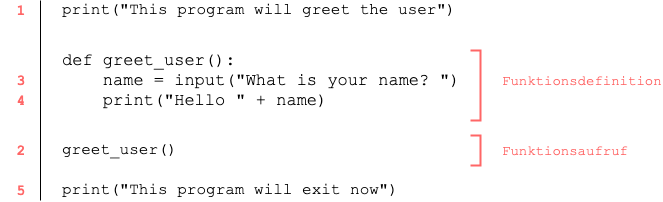
\includegraphics[width=0.8\linewidth,height=0.8\textheight,keepaspectratio]{chapters/09_python3_control_flow/figures/function-flow.png}
                \caption{Der Programmablauf beim Aufruf einer Funktion. Die Ausführungsreihenfolge der einzelnen Anweisungen ist links in rot dargestellt.}
                \label{fig:function-flow}
            \end{figure}
    \end{frame}
    
    \begin{frame}[fragile]{Funktionsaufruf (III)}
        \begin{alertblock}{Achtung}
            Beim Aufruf einer Funktion muss immer sichergestellt sein, dass die Funktion zum Zeitpunkt des Aufrufs bereits bekannt ist. Folgender Codeabschnitt würde also einen Fehler erzeugen, da die Funktion aufgerufen wird, bevor sie definiert wurde.
            
\begin{pythoncode}
greet_user()

def greet_user():
    name = input("What is your name? ")
    print("Hello " + name) 
\end{pythoncode}
        \end{alertblock}
    \end{frame}
    
    
    \begin{frame}{Parameter \& Argumente (I)}
        In vielen Fällen werden von Funktionen zusätzliche Informationen erwartet, die beispielsweise lediglich in Variablen außerhalb der Funktion existieren und daher im Rumpf der Funktion nicht zugänglich sind. \\~\
        
        Hierfür können den Funktionen zusätzliche Daten übergeben werden, welche dann innerhalb der Funktionsausführung genutzt werden können. Diese Daten müssen sowohl bei der Definition als auch dem Aufruf von Funktionen berücksichtigt werden. \\~\
        
        Sowohl Parameter als auch Argumente werden jeweils durch Komma getrennt.
    \end{frame}
    
    \begin{frame}[fragile]{Funktionsdefinition - Parameter (I)}
        Bei der Funktionsdefinition muss angegeben werden, welche bzw. wie viele Daten erwartet werden. Diese Werte werden dann einem Variablennamen zugewiesen, der lediglich innerhalb der Funktion (Scope) existiert. Sobald die Funktion abgearbeitet wurde und im Ablauf aus der Funktion gesprungen wird, sind dem Interpreter die zugewiesenen Werte nicht mehr bekannt. \\~\
        
        Die Werte, die von einer Funktion erwartet werden, heißen \textbf{Parameter}.
        
    \end{frame}
    
    \begin{frame}[fragile]{Funktionsdefinition - Parameter (II)}
        \begin{exampleblock}{Beispiel}
            In diesem Codeabschnitt werden der Funktion \code{add} zwei Werte übergeben, nämlich die zwei Summanden. Diese Werte können innerhalb der Funktion mithilfe der Variablen \code{summand1} und \code{summand2} verwendet werden. Diese beiden Werte sind die Parameter, die beim Aufruf der Funktion übergeben werden müssen. 
            
            Die Bezeichnung der Parameter ist dem Entwickler selbst überlassen, die Parameternamen sollten jedoch ebenso wie normale Variablen möglichst aussagekräftig sein.
            
\begin{pythoncode}
def add(summand1, summand2):
    sum = summand1 + summand2
    print("The result of " + summand1 + " + " + summand2 + " is " + sum)
\end{pythoncode}
        \end{exampleblock}
    \end{frame}
    
    \begin{frame}{Funktionsaufruf - Argumente (I)}
        Falls eine Funktion per ihrer Definition Werte erwartet, wie im vorherigen Beispiel die \code{add}-Funktion, so müssen die konkreten Werte beim Aufruf der Funktion zwangsläufig mit übergeben werden. \\~\
        
        Wird also die \code{add}-Funktion aufgerufen, müssen zwei Werte (die beiden Summanden) übergeben werden. Die konkreten Werte, die beim Funktionsaufruf an die Funktionsdefinition übergeben werden, heißen \textbf{Argumente}.
    \end{frame}
    
        \begin{frame}[fragile]{Funktionsaufruf - Argumente (II)}
        \begin{exampleblock}{Beispiel}
            In diesem Codeabschnitt wird die Funktion \code{add} mit den beiden Summanden 3 und 5 aufgerufen. 3 und 5 sind also die Argumente, die der \code{add} Funktion übergeben werden. \\~\
            
            Innerhalb der \code{add}-Funktion können die beiden Argumente mithilfe der Variablennamen \code{summand1} und \code{summand2} verwendet werden
            
\begin{pythoncode}
def add(summand1, summand2):
    sum = summand1 + summand2
    print("The result of " + summand1 + " + " + summand2 + " is " + sum)
    

add(3,5)
\end{pythoncode}

\begin{pythoncode}
The result of 3 + 5 is 8
\end{pythoncode}
        \end{exampleblock}
    \end{frame}
    
    
    \begin{frame}[fragile]{Parameter \& Argumente (II)}
        Im Normalfall muss die Anzahl der Parameter immer der Anzahl der Argumente entsprechen. \\~\
        
        Werden weniger Argumente übergeben als Parameter definiert wurden, sind ein oder mehrere Werte unbesetzt, woraufhin der Interpreter einen Fehler wirft:
\begin{pythoncode}
add(3)
TypeError: add() missing 1 required positional argument: 'summand2'
\end{pythoncode} \\~\

       Werden mehr Argumente übergeben als Parameter definiert, kann die Funktion auch nicht ausgeführt werden:
       
\begin{pythoncode}
add(3,5,2)
TypeError: add() takes 2 positional arguments but 3 were given
\end{pythoncode}
    \end{frame}
    
    
    \begin{frame}[fragile]{Function Overloading (I)}
        \begin{alertblock}{Achtung}
            Es ist in Python nicht möglich, zwei oder mehr unterschiedliche Funktionen mit gleichem Namen und gleicher Anzahl von Parametern aufzurufen, da die Funktionen anhand ihres Funktionskopfes nicht eindeutig unterscheidbar sind. \\~\
            
            Es ist aber möglich, zwei oder mehr Funktionen mit gleichem Namen aber unterschiedlicher Anzahl an Parametern zu definieren, da beim Aufruf anhand der Anzahl der übergebenen Argumente darauf geschlossen werden kann, welche der Funktionen ausgeführt werden soll. \\~\
            
            Dies wird als \textbf{Overlaoding} (bzw. Überladen) von Funktionen bezeichnet.
        \end{alertblock}
    \end{frame}
    
    \begin{frame}[fragile]{Function Overloading (II)}
        \begin{exampleblock}{Beispiel}
            In diesem Beispiel wird die erste \code{add}-Funktion durch die zweite Funktion überschrieben, sodass letztendlich nur eine \code{add}-Funktion existiert.
\begin{pythoncode}
def add(summand1, summand2):
    print("Result of 1st function: " + str(summand1 + summand2))

def add(addend1, addend2):
    print("Result of 2nd function: " + str(addend1 + addend2))
\end{pythoncode}

        In diesem Beispiel koexistieren beide Funktionen, da sie eindeutig unterscheidbar sind:
\begin{pythoncode}
def add(summand1, summand2):
    print("Result of 1st function: " + str(summand1 + summand2))

def add(summand1, summand2, summand3):
    print("Result of 2nd function: " + str(summand1 + summand2 + summand3))
\end{pythoncode}        
        \end{exampleblock}
    \end{frame}
    
    \begin{frame}[fragile]{Keyword Argumente (I)}
        Standardmäßig entspricht die Reihenfolge der übergebenen Argumente der Reihenfolge der Parameter, d.h. im obigen Beispiel wird das erste Argument \code{3} dem Parameter \code{summand1} und das zweite Argument \code{5} dem Parameter \code{summand2} zugewiesen. \\~\
        
        Um dies noch offensichtlicher bzw. expliziter zu machen, können die Argumente auch zusammen mit der Parameterbezeichnung (mit \code{=} verbunden) übergeben werden, was als \textit{Keyword Argumente} bezeichnet wird:
        
\begin{pythoncode}
def add(summand1, summand2):
    sum = summand1 + summand2
    print("The result of " + summand1 + " + " + summand2 + " is " + sum)
    

add(summand1=3, summand2=5)

The result of 3 + 5 is 8
\end{pythoncode}
    \end{frame}
    
    \begin{frame}[fragile]{Keyword Argumente (II)}
        Auf diese Weise ist es auch möglich, die Reihenfolge der Argumente zu ändern (was jedoch vermieden werden sollte, da es der Übersichtlichkeit und einfachen Lesbarkeit des Codes widerspricht).
        
\begin{pythoncode}
def add(summand1, summand2):
    sum = summand1 + summand2
    print("The result of " + summand1 + " + " + summand2 + " is " + sum)
    

add(summand2=5, summand1=3)

The result of 3 + 5 is 8
\end{pythoncode}

        Obwohl hier der Summand 2 als erstes und Summand 1 als zweites übergeben wurden, wurden sie anhand der Parameter-Keywords trotzdem richtig zugeordnet.
    \end{frame}
    
    \begin{frame}[fragile]{Default Argumente (I)}
        Es ist auch möglich, einer Funktion weniger Argumente zu übergeben als Parameter definiert wurden, sofern die fehlenden Parameter Standardwerte besitzen. \\~\
        
        Bei der Definition von Funktionen könnnen nämlich für die Parameter Standardwerte angegeben werden, die verwendet werden, wenn für den jeweiligen Parameter kein Argument übergeben wurde. Ist ist aber auch möglich, ein Argument für einen Parameter zu übergeben, für den ein Standardwert definiert wurde. In diesem Fall wird der Standardwert ignoriert und der übergebene Argumentwert genutzt.
        
        
    \end{frame}
    
    \begin{frame}[fragile]{Default Argumente (II)}
        \begin{exampleblock}{Beispiel}
\begin{pythoncode}

def greet_user(name="stranger"):
    print("Hello, nice to meet you, " + name)
\end{pythoncode}

Falls der Nutzer für den \code{name}-Parameter ein Argument übergibt, so wird dieses verwendet:
\begin{pythoncode}
greet_user("Alice")
"Hello, nice to meet you, Alice"
\end{pythoncode}

Wird kein Argument übergeben, so wird der Standardwert ("stranger") verwendet:
\begin{pythoncode}
greet_user()
"Hello, nice to meet you, stranger"
\end{pythoncode}
        \end{exampleblock}
    \end{frame}
    
    \begin{frame}[fragile]{Default Argumente (III)}
        \begin{alertblock}{Achtung}
            Standardargumente müssen in der Funktionsdefinition immer \textbf{nach} den Pflichtargumenten stehen, da andernfalls ein Fehler geworfen wird.\\~\
            
            Folgendes ist also nicht möglich:
\begin{pythoncode}
def check_legal_age(legal_age=18, user_age):
    if user_age >= legal_age:
        print("User is full-age")
    else:
        print("User is under full-age")

SyntaxError: non-default argument follows default argument
\end{pythoncode}

        Korrekt ist der Funktionskopf folgendermaßen:
\begin{pythoncode}
def check_legal_age(user_age, legal_age=18):
    ...
\end{pythoncode}        
        \end{alertblock}
    \end{frame}
    
    
    \begin{frame}[fragile]{Rückgabewerte (I)}
        Häufig werden Funktionen genutzt, um wiederkehrende Berechnungen mit unterschiedlichen Argumenten durchzuführen. \\~\
        
        Das Problem der bisher gezeigten Funktionen besteht darin, dass die Funktionen inhaltlich vom aufrufenden Code abgekapselt sind. Werte bzw. Variablen, die innerhalb einer Funktion erzeugt werden, sind nur innerhalb des jeweiligen Funktionsrumpfes gültig (\textit{Scoping}). Wird beispielsweise innerhalb einer Funktion eine Summe berechnet und in einer Variablen gespeichert, ist die Variable außerhalb der Funktion nicht "sichtbar".

\begin{pythoncode}
def add(summand1, summand2):
    calculated_sum = summand1 + summand2

add(3,5)
print(calculated_sum)

NameError: name 'calculated_sum' is not defined
\end{pythoncode}
    \end{frame}
    
    \begin{frame}[fragile]{Rückgabewerte (II)}
        Jedoch sind genau diese Werte, die innerhalb von Funktionen berechnet werden, für die Entwicklung von Bedeutung, da diese Ergebnisse beispielsweise auch außerhalb der Funktionen für den jeweils folgenden Codeablauf benötigt werden. \\~\
        
        Daher können Werte von Funktionen an die aufrufende Stelle zurückgeben, diese Werte werden als \textbf{Rückgabewerte} bzw. \textbf{Return Values} bezeichnet.\\~\
        
        Sie können analog zu Argumenten verstanden werden, die als Eingabewerte für Funktionen genutzt werden. Anstatt Werte von außerhalb innerhalb des Funktionsrumpfs verfügbar zu machen werden durch Rückgabewerte Variablen innerhalb des Funktionsrumpfs außerhalb verfügbar gemacht.
    
    \end{frame}
    
    \begin{frame}[fragile]{Rückgabewerte (III)}
        Rückgabewerte werden durch das \code{return} Schlüsselwort an die Stelle zurückgegeben, an der die Funktion aufgerufen wurde. Dort kann der Wert beispielsweise in einer Variable gespeichert werden.
        
        \begin{exampleblock}{Beispiel}
            Im folgenden Beispiel wird innerhalb der \code{add}-Funktion eine Summe gebildet und in der \code{calculated\_sum}-Variable gespeichert. Diese wird anschließend zurückgegeben an die Stelle, an die die Funktion aufgerufen wurde. Der Wert von \code{calculated\_sum} wird also außerhalb der Funktion in der Variablen \code{result} gespeichert.
\begin{pythoncode}
def add(summand1, summand2):
    calculated_sum = summand1 + summand2
    return calculated_sum

result = add(3,5)
print(result)
8
\end{pythoncode}        
        \end{exampleblock}
    \end{frame}
    
    \begin{frame}[fragile]{Rückgabewerte (IV)}
    
        Jede Funktion in Python gibt einen Wert zurück. Auch in den zuvor gezeigten Funktionen ohne explizite \code{return}-Anweisung wird ein Wert zurückgegeben.
        
        Falls die Ausführung einer Funktion am Ende angelangt ist und kein \code{return}-Statement existiert, wird standardmäßig der Wert \code{None} zurückgegeben.

\begin{pyconcode}
>>> def add(summand1, summand2):
...     calculated_sum = summand1 + summand2
    
>>> result = add(3,5)

>>> print(result)
None

>>> print(type(result))
<class 'NoneType'>

\end{pyconcode}
    \end{frame}
    
    \begin{frame}[fragile]{Rückgabewerte (V)}
        \begin{alertblock}{Achtung}
            Durch das \code{return}-Keyword wird die Ausführung einer Funktion immer abgebrochen und es wird zur Stelle des Funktionsaufrufs zurückgesprungen. Daher macht es keinen Sinn, wenn eine Funktion nach einem \code{return}-Statement weiteren Code enthält, da dieser ignoriert wird.
            
\begin{pythoncode}
def add(summand1, summand2):
    calculated_sum = summand1 + summand2
    return calculated_sum
    
    print(calculated_sum) # Dieser Code wird nicht ausgeführt
\end{pythoncode}
        \end{alertblock}
    \end{frame}
    
    
    \begin{frame}[fragile]{pass}
        Manchmal soll zwar eine Funktion bereits definiert werden, jedoch soll der Funktionsrumpf erst später implementiert werden. In solchen Fällen ist es nicht erlaubt, nur den Funktionskopf aufzuführen und den Rumpf leer zu lassen, da Python, um den Beginn und das Ende der Funktion zu erkennen, einen eingerückten Block erwartet.
        
\begin{pythoncode}
def add(summand1, summand2):

IndentationError: expected an indented block
\end{pythoncode}

        Um den Rumpf dennoch leer zu lassen und keinen Fehler zu erzeugen, kann das Platzhalter-Schlüsselwort \code{pass} genutzt werden. Es besitzt keinerlei Funktionalität, sondern dient nur dazu, einen (eingerückten) Block zu kennzeichnen, der eigentlich leer ist.

        
\begin{pythoncode}
def add(summand1, summand2):
    pass
\end{pythoncode}
    \end{frame}
    
    \begin{subsection}{Aufgaben}
        \begin{frame}[fragile, allowframebreaks]{Aufgaben}
            \begin{enumerate}
                \item Wozu werden Funktionen genutzt / benötigt?
                \item Aus welchen 3 Teilen bestehen Funktionen?
                \item Worin besteht der Unterschied zwischen Built-in Funktionen und eigenen Funktionen?
                \item Worauf muss beim Aufruf von Funktionen prinzipiell geachtet werden?
                \item Worin unterscheiden sich Funktionsdefinitionen und -aufrufe?
                \item Worin besteht der Unterschied zwischen Parametern und Argumenten?
            \end{enumerate}
        \end{frame}
    \end{subsection}
    
\section{Module}
    \label{subs:modules}
    
    \begin{frame}{Module (I)}
        Da insbesondere bei umfangreichen Projekten der Codeumfang sehr groß sein kann, ist es schwierig, die Übersichtlichkeit zu wahren und die Komplexität in der Struktur gering zu halten.\\~\
        
        Den gesamten Code in einer einzigen Datei zu verwalten ist zwar für simple Projekte oder einfache Skripte ausreichend, für umfangreiche Arbeiten sollte dies aber vermieden werden.
    \end{frame}
    
    \begin{frame}{Module (II)}
        Aus diesem Grund stehen in Python, wie in vielen anderen (modernen) Programmiersprachen auch, sogenannte \textbf{Module} zur Verfügung.\footnote{Die Bezeichnung kann sich zwischen den Programmiersprachen unterscheiden, z.B. \textit{Pakete}, \textit{Container}, ... } \\~\
        
        Diese helfen dabei, den Code zu gliedern, strukturieren und separieren. So können zusammengehörige Funktionalitäten in gleichen Modulen untergebracht werden, während Funktionalitäten, die sich auf eine andere Domäne oder ein anderes Anwendungsgebiet beziehen, in andere, separate Module gegliedert werden.
    \end{frame}
    
    \begin{frame}[fragile]{Module (III)}
        Funktionen und Variablen, die sich in Modulen befinden, können in anderen Dateien/Modulen importiert werden. Nachdem sie importiert wurden, stehen sie ganz normal in der jeweiligen Datei zur Verfügung. Sie verhalten sich also so, als wären sie in der aktuellen Datei enthalten.\\~\
        
        Hierzu wird das \code{import}-Keyword genutzt. \\~\
        
        Ein Modul besitzt den Namen der Datei, in der die Anweisungen gespeichert sind. Falls die Datei also \code{calculations.py} heißt, kann das Modul mit dem Namen \code{calculations} importiert werden:
        
\begin{pythoncode}
import calculations
\end{pythoncode}
    \end{frame}
    
    \begin{frame}[fragile]{Module (IV)}
        Nachdem das Modul importiert wurde, sind die darin enthaltenen Funktionen und Anweisungen mit einem Punkt getrennt aufrufbar.\\~\
        
        Falls also folgendes in der Datei \code{calculations.py} enthalten ist:

\begin{pythoncode}
def add(summand1, summand2):
    return summand1 + summand2
\end{pythoncode}

    dann kann der Code in einer anderen Datei folgendermaßen ausgeführt werden:
    
\begin{pythoncode}
import calculations

calculations.add(3,5)
\end{pythoncode}
    \end{frame}
    
    \begin{frame}[fragile, allowframebreaks]{Built-in Module}
    
        Ebenso wie bei Funktionen gibt es auch Module, die bereits im Python-Interpreter vorhanden sind und vom Entwickler genutzt werden können. Entsprechend der Trennung der Funktionalitäten sind die Funktionalitäten gegliedert, z.B existieren folgende Module:
        
        \begin{itemize}
            \item \textbf{math}: Mathematische Funktionen wie \code{math.floor()}, \code{math.log()}, \code{math.tan()}, ...
            \item \textbf{time}: Funktionen zur Verarbeitung von Zeiten, Datumsangaben u.ä. wie \code{time.time()}, \code{time.sleep()}, ...
            \item \textbf{os}: Modul für plattformunabhängige Funktionalitäten wie \code{os.getlogin()}, \code{os.mkdir()}
            \item \textbf{sqlite3}: Funktionen zum Zugriff auf SQLite-Datenbanken wie \code{sqlite3.connect()}, \code{sqlite3.close()}, ...
            \item \textbf{threading} und multiprocessing : Funktionalitäten zum (Multi-)Threading und (Multi-)Processing wie \code{threading.main\_thread()}, \code{multiprocessing.Process.run()}
            \item \textbf{json}: Modul für JSON-Funktionalitäten wie \code{json.load()}, \code{json.dump()}
            \item \textbf{http}: Modul, das mehrere Untermodule für Funktionalitäten bezogen auf HTTP enthält wie \code{http.client}, \code{http.server}, ...
            \item viele weitere (siehe \href{https://docs.python.org/3/library/}{Docs})
        \end{itemize}
        
        \begin{exampleblock}{Beispiel}
\begin{pyconcode}
>>> import math
>>> import time

>>> print(math.log(1))
0.0

>>> print(time.time())
1580846245.522497
\end{pyconcode}
        \end{exampleblock}
    \end{frame}
%\section{Objektorientierung}